\documentclass[12pt]{beamer}

\usepackage[utf8]{inputenc}
\usepackage{listings}
\usepackage{tikz}
\usepackage{amsmath}

\lstset{language=C++, basicstyle=\footnotesize, frame=single}

\beamertemplatenavigationsymbolsempty
\AtBeginSection[]
{
    \begin{frame}
    \frametitle{Table of Contents}
    \tableofcontents[currentsection]
    \end{frame}
}

\title{Game theory}
\subtitle{Nim game, Minimax, Alpha-Beta pruning}
\author{beOI Training}
\institute{
\includegraphics[height=12em]{../share/beoi-logo}}

\begin{document}

\maketitle


\section{Basics and decision trees}
\begin{frame}
\frametitle{What is game theory?}
Modelling strategic situations:
\begin{itemize}
\item with conflict or cooperation
\begin{itemize} \item chess, football, pictionary, ... \end{itemize}
\item decisions based on personal goals
\begin{itemize} \item beating the opponent, maximizing points, ... \end{itemize}
\item influenced by the choice patterns of other players
\begin{itemize} \item if someone plays predictably, you can use it against them \end{itemize}
\item might involve randomness
\begin{itemize} \item dice rolls, card draws, ... \end{itemize}
\end{itemize}

~

Goal: compute choices, optimal strategies, expected gains
\end{frame}

\begin{frame}
\frametitle{Decision trees}
A useful tool to examine decisions and their consequences.
\begin{center}
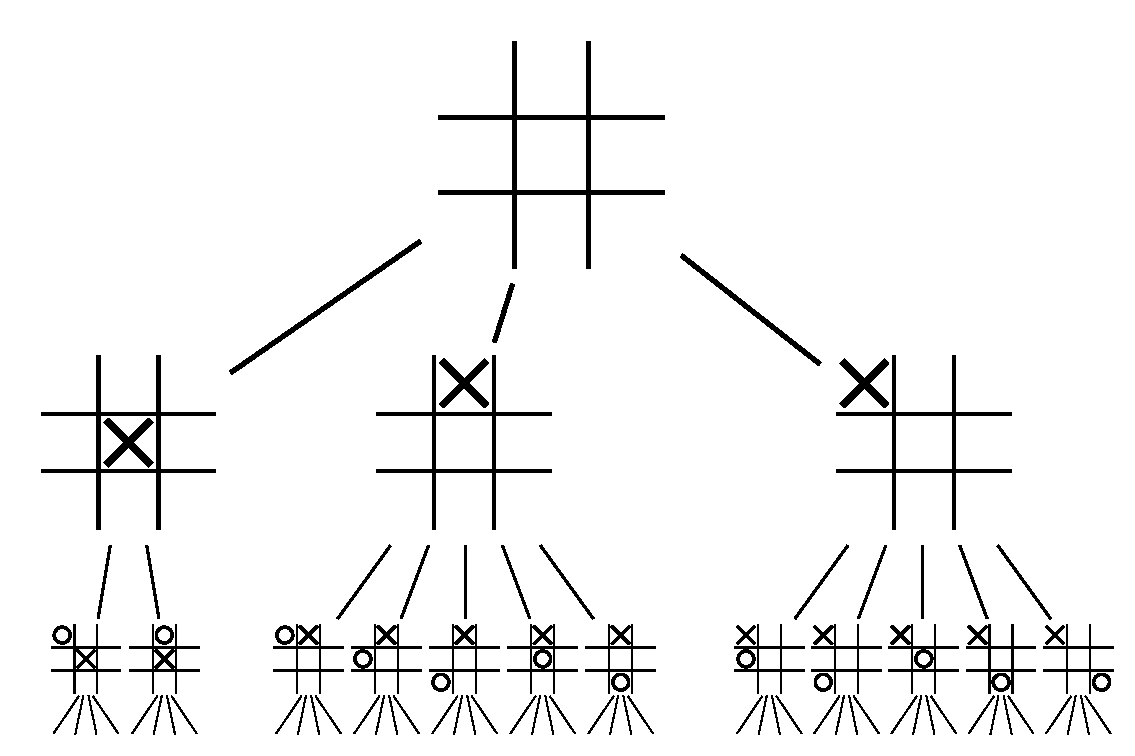
\includegraphics[width=.95\linewidth]{img/tictactoe}
\end{center}
\end{frame}

\begin{frame}
\frametitle{Utility vectors and zero-sum games}
Utility vectors:
\begin{itemize}
\item define the ``gains'' of an end state
\item one entry per player: $(2,3,-2)$, $(0,7)$, ...
\item determine the choices of players
\begin{itemize} \item player 1 will choose $({\bf 3},5)$ over $({\bf 2},3)$ \end{itemize}
\item but not always!
\begin{itemize} \item should player 2 choose $(0,{\bf 6},5)$ or $(2,{\bf 6},3)$? \end{itemize}
\end{itemize}

~

Main focus: two-player zero-sum games:
\begin{itemize}
\item only two players: no complicated interactions
\item zero-sum: our benefits are the opponent's losses
\begin{itemize} \item $(5,-5)$, $(-3,3)$, $(0,0)$, ... (or just $5$, $-3$, $0$) \end{itemize}
\item the value of a choice is always well-defined
\end{itemize}
\end{frame}


\section{Subtraction game}
\begin{frame}
\frametitle{Subtraction game: rules}
\end{frame}

\begin{frame}
\frametitle{Subtraction game: decision tree}
\end{frame}

\begin{frame}
\frametitle{Subtraction game: winning states}
\end{frame}

\begin{frame}
\frametitle{Subtraction game: optimal play}
\end{frame}


\section{Nim game}

\begin{frame}
\frametitle{Nim game: rules}
\end{frame}

\begin{frame}
\frametitle{Nim game: two stacks}
\end{frame}

\begin{frame}
\frametitle{Nim game: key invariant}
\end{frame}

\begin{frame}
\frametitle{Nim game: losing situation}
\end{frame}

\begin{frame}
\frametitle{Nim game: winning situation}
\end{frame}


\section{Minimax algorithm}
\begin{frame}
\frametitle{Minimax principles}
\end{frame}

\begin{frame}
\frametitle{Minimax example}
\end{frame}

\begin{frame}
\frametitle{Minimax implementation}
\end{frame}

\begin{frame}
\frametitle{Minimax with DP}
\end{frame}

\section{Alpha-Beta pruning}
\begin{frame}
\frametitle{Very large search spaces}
\end{frame}

\begin{frame}
\frametitle{Alpha-beta definition}
\end{frame}

\begin{frame}
\frametitle{Alpha-beta example}
\end{frame}

\begin{frame}
\frametitle{Alpha-beta implementation}
\end{frame}

\begin{frame}
\frametitle{Sources of figures}
\begin{itemize}
\item \url{https://commons.wikimedia.org/wiki/File:Tic-tac-toe-game-tree.svg}
\end{itemize}
\end{frame}

\end{document}
